\section{Experiment}
\label{experiment}


\subsection{Network Setup and Launch Attack}

In this part of research, we cover introduction of our testing environment and also experimental setup of those machines. We have installed and configured three Virtual Machines - Victim, Attacker and Vulnerable. All virtual machines are run on the same individual server, but they are separate in logical. The traffic flow between each machines are shown in Figure \ref{fig:connectionModel}. In which victim's VM configured with snort, attacker's machine contains Metasploit tool-kit and we used existing vulnerable Ubuntu operating system for testing purposes and make it as our third machine - vulnerable \cite{misc:metasploitable}. We have deployed and tested ten different Metasploit attacks and we divided it into three types of attack including Port Scanning (Probe) - gathering network information to bypass security, Denial of Service (Dos) - where some resource is swamped; causing DoS to legitimate users, Remote to local (R2L) - attacks that exploit remote system vulnerabilities to get access to a system. After successfully tested we made all of them as automated handled by Metasploit script, which we used for development of attacker's system\cite{misc:metasploitScripts}.


\begin{figure}[h!]
	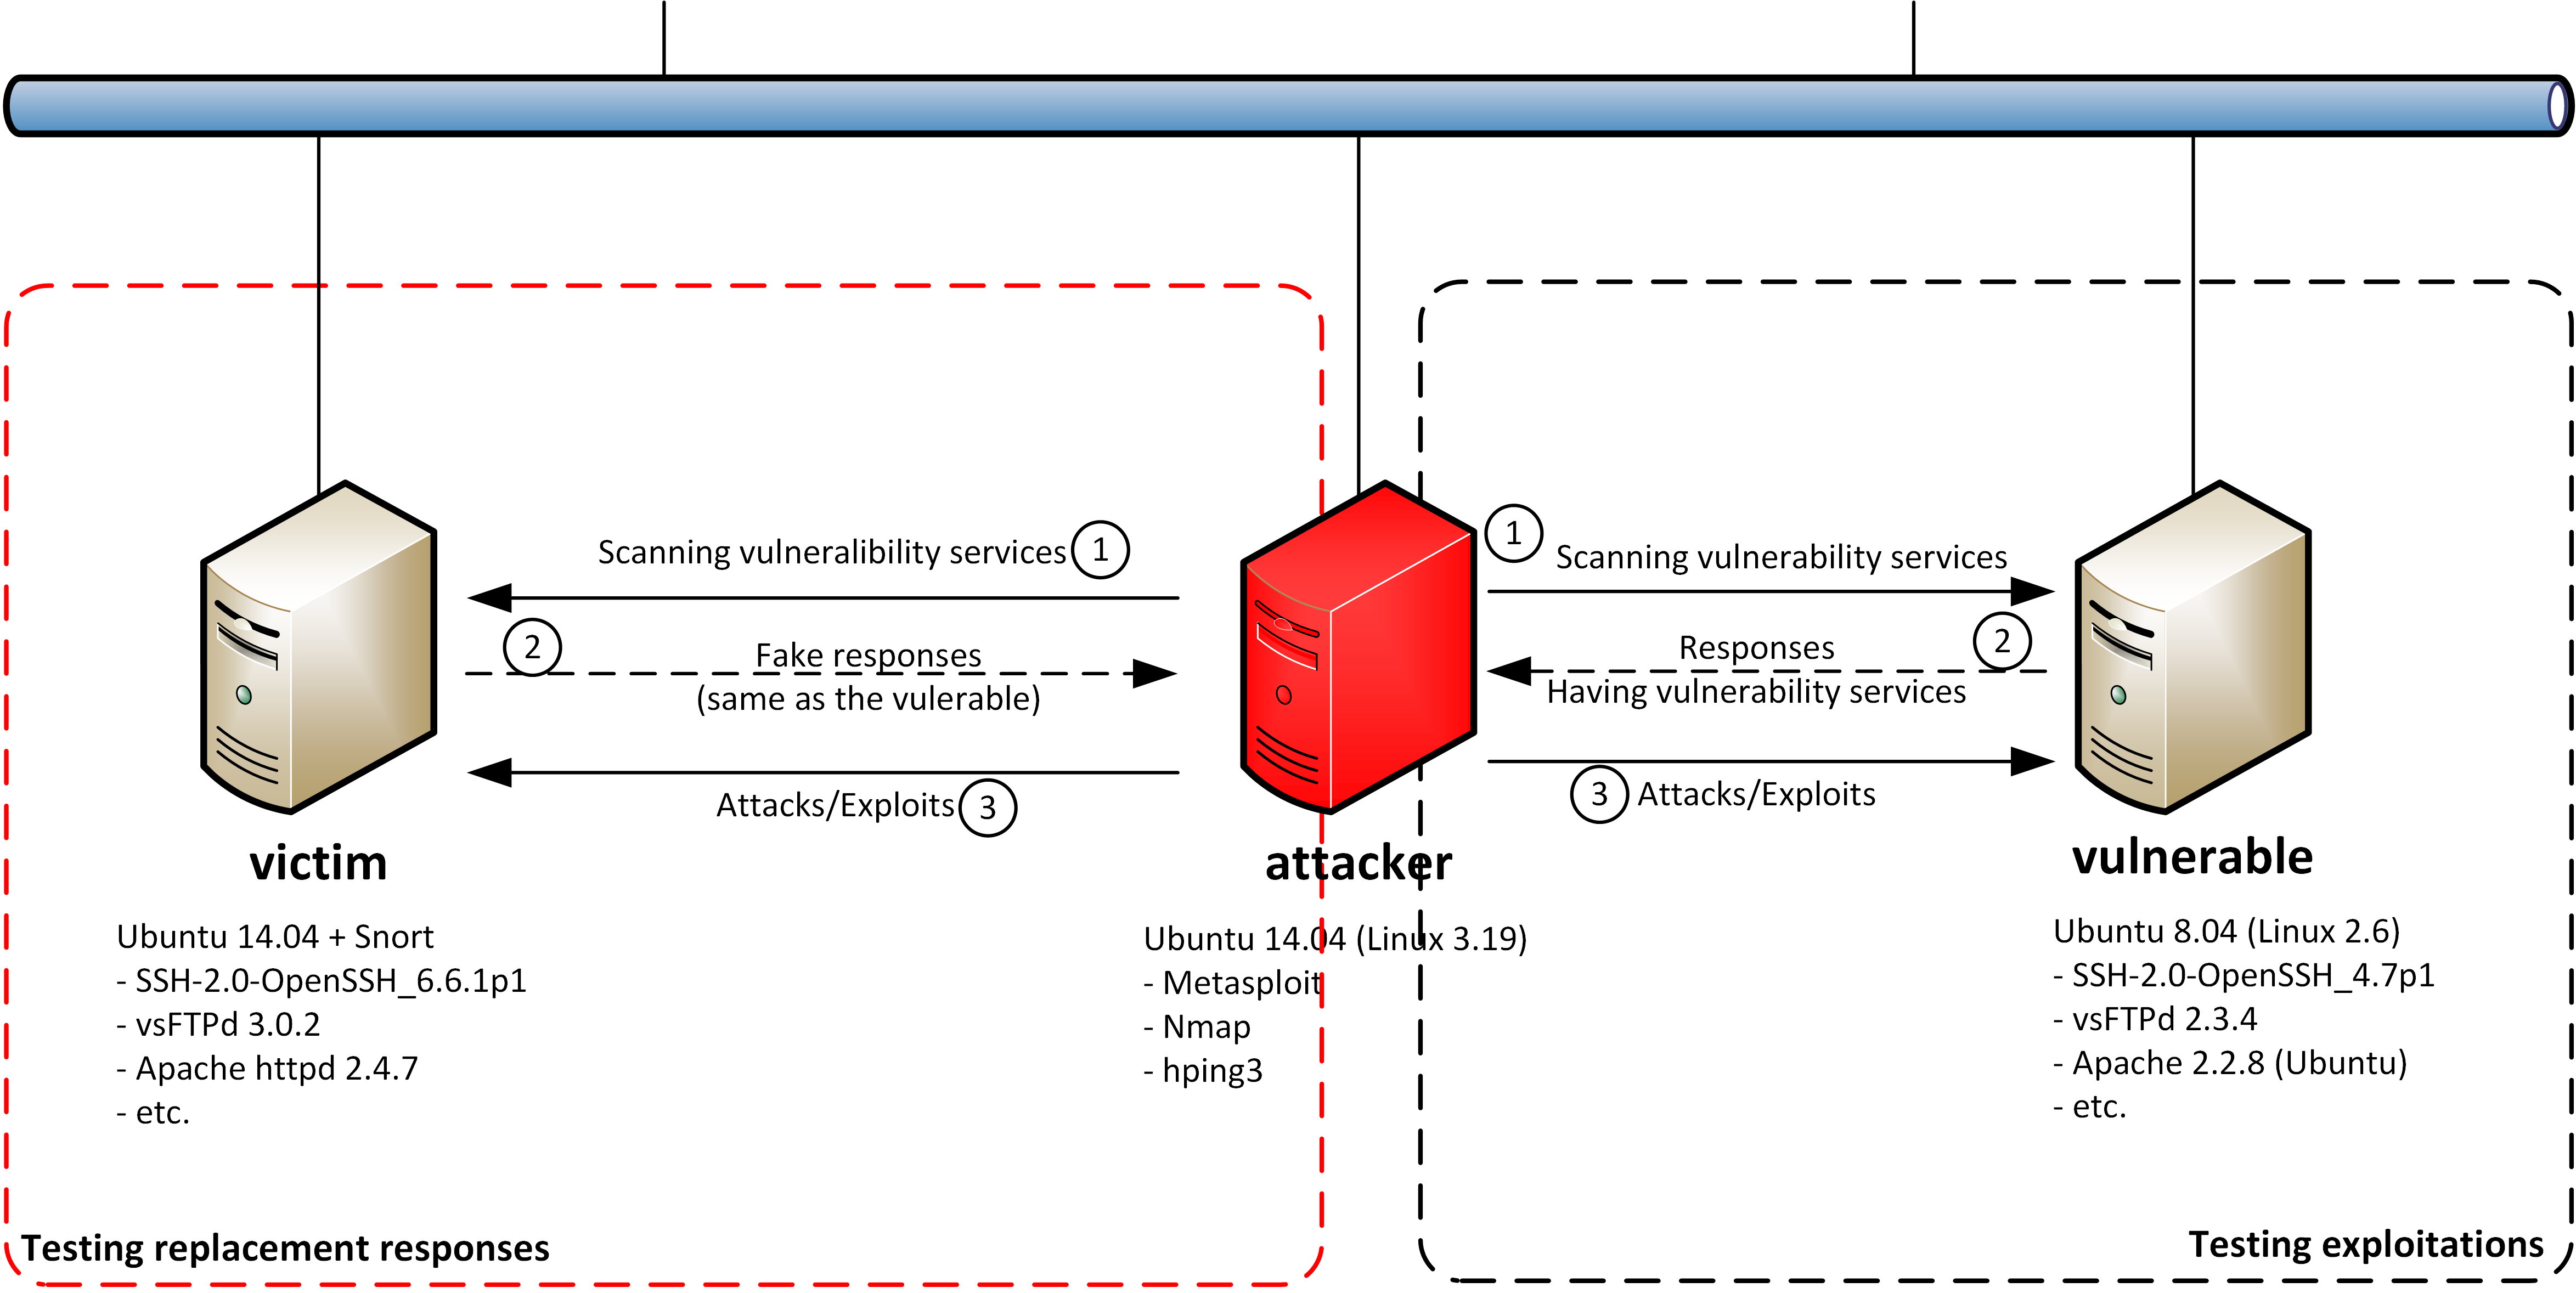
\includegraphics[width=\linewidth]{networkSecurityResearch_new_no_back.png}
	\caption{Logical connection model}
	\label{fig:connectionModel}
\end{figure}

\subsection{Dataset preparation}

%We started research to work on dataset preparation by taking existing dataset and run their suggested machine learning techniques using weka tool. And when we were %working on KDD- cup'99 dataset we found it was really outdated as it was to older and those number of features which they have focused on, it was not applicable with %our research because we focused on network threat as we were looking at network behavior and traffic for anomaly detection for intrusion detection %system\cite{anomaly-basedNID}. 

In this part of research to collect and extract dataset we started data modeling with existing different labeled datasets to understand the model of machine learning. Then we worked on existing datasets to extract usable features from it and we came up with the java parser script which can parse and extract entire data information from Pcap file and saved into Csv file. We put time-window size variable to extract and identify unique combinations of packet transmission. Parser can parse and split the entire Pcap information with respect to the time-window size. While researching on previous suggested approaches we tried to extract dataset by different time-windows size by changing its value by 10 seconds, 1 seconds, 7 seconds, and 5 seconds. We observe that 4 second time frame is more preferable in our network architecture as it generate more accurate result with weka. As this feature is flexible and it is depends on the nodes in our network. We collected and built our own datasets to test our model and accuracy of algorithms for anomaly detection of network attacks \cite{DMnIDS}. We launch each attack repeatedly and capture those Pcap and after merging those Pcap we extract that into Csv format using our own Csv-parser by 4 second time window size.

\begin{figure}[h!]
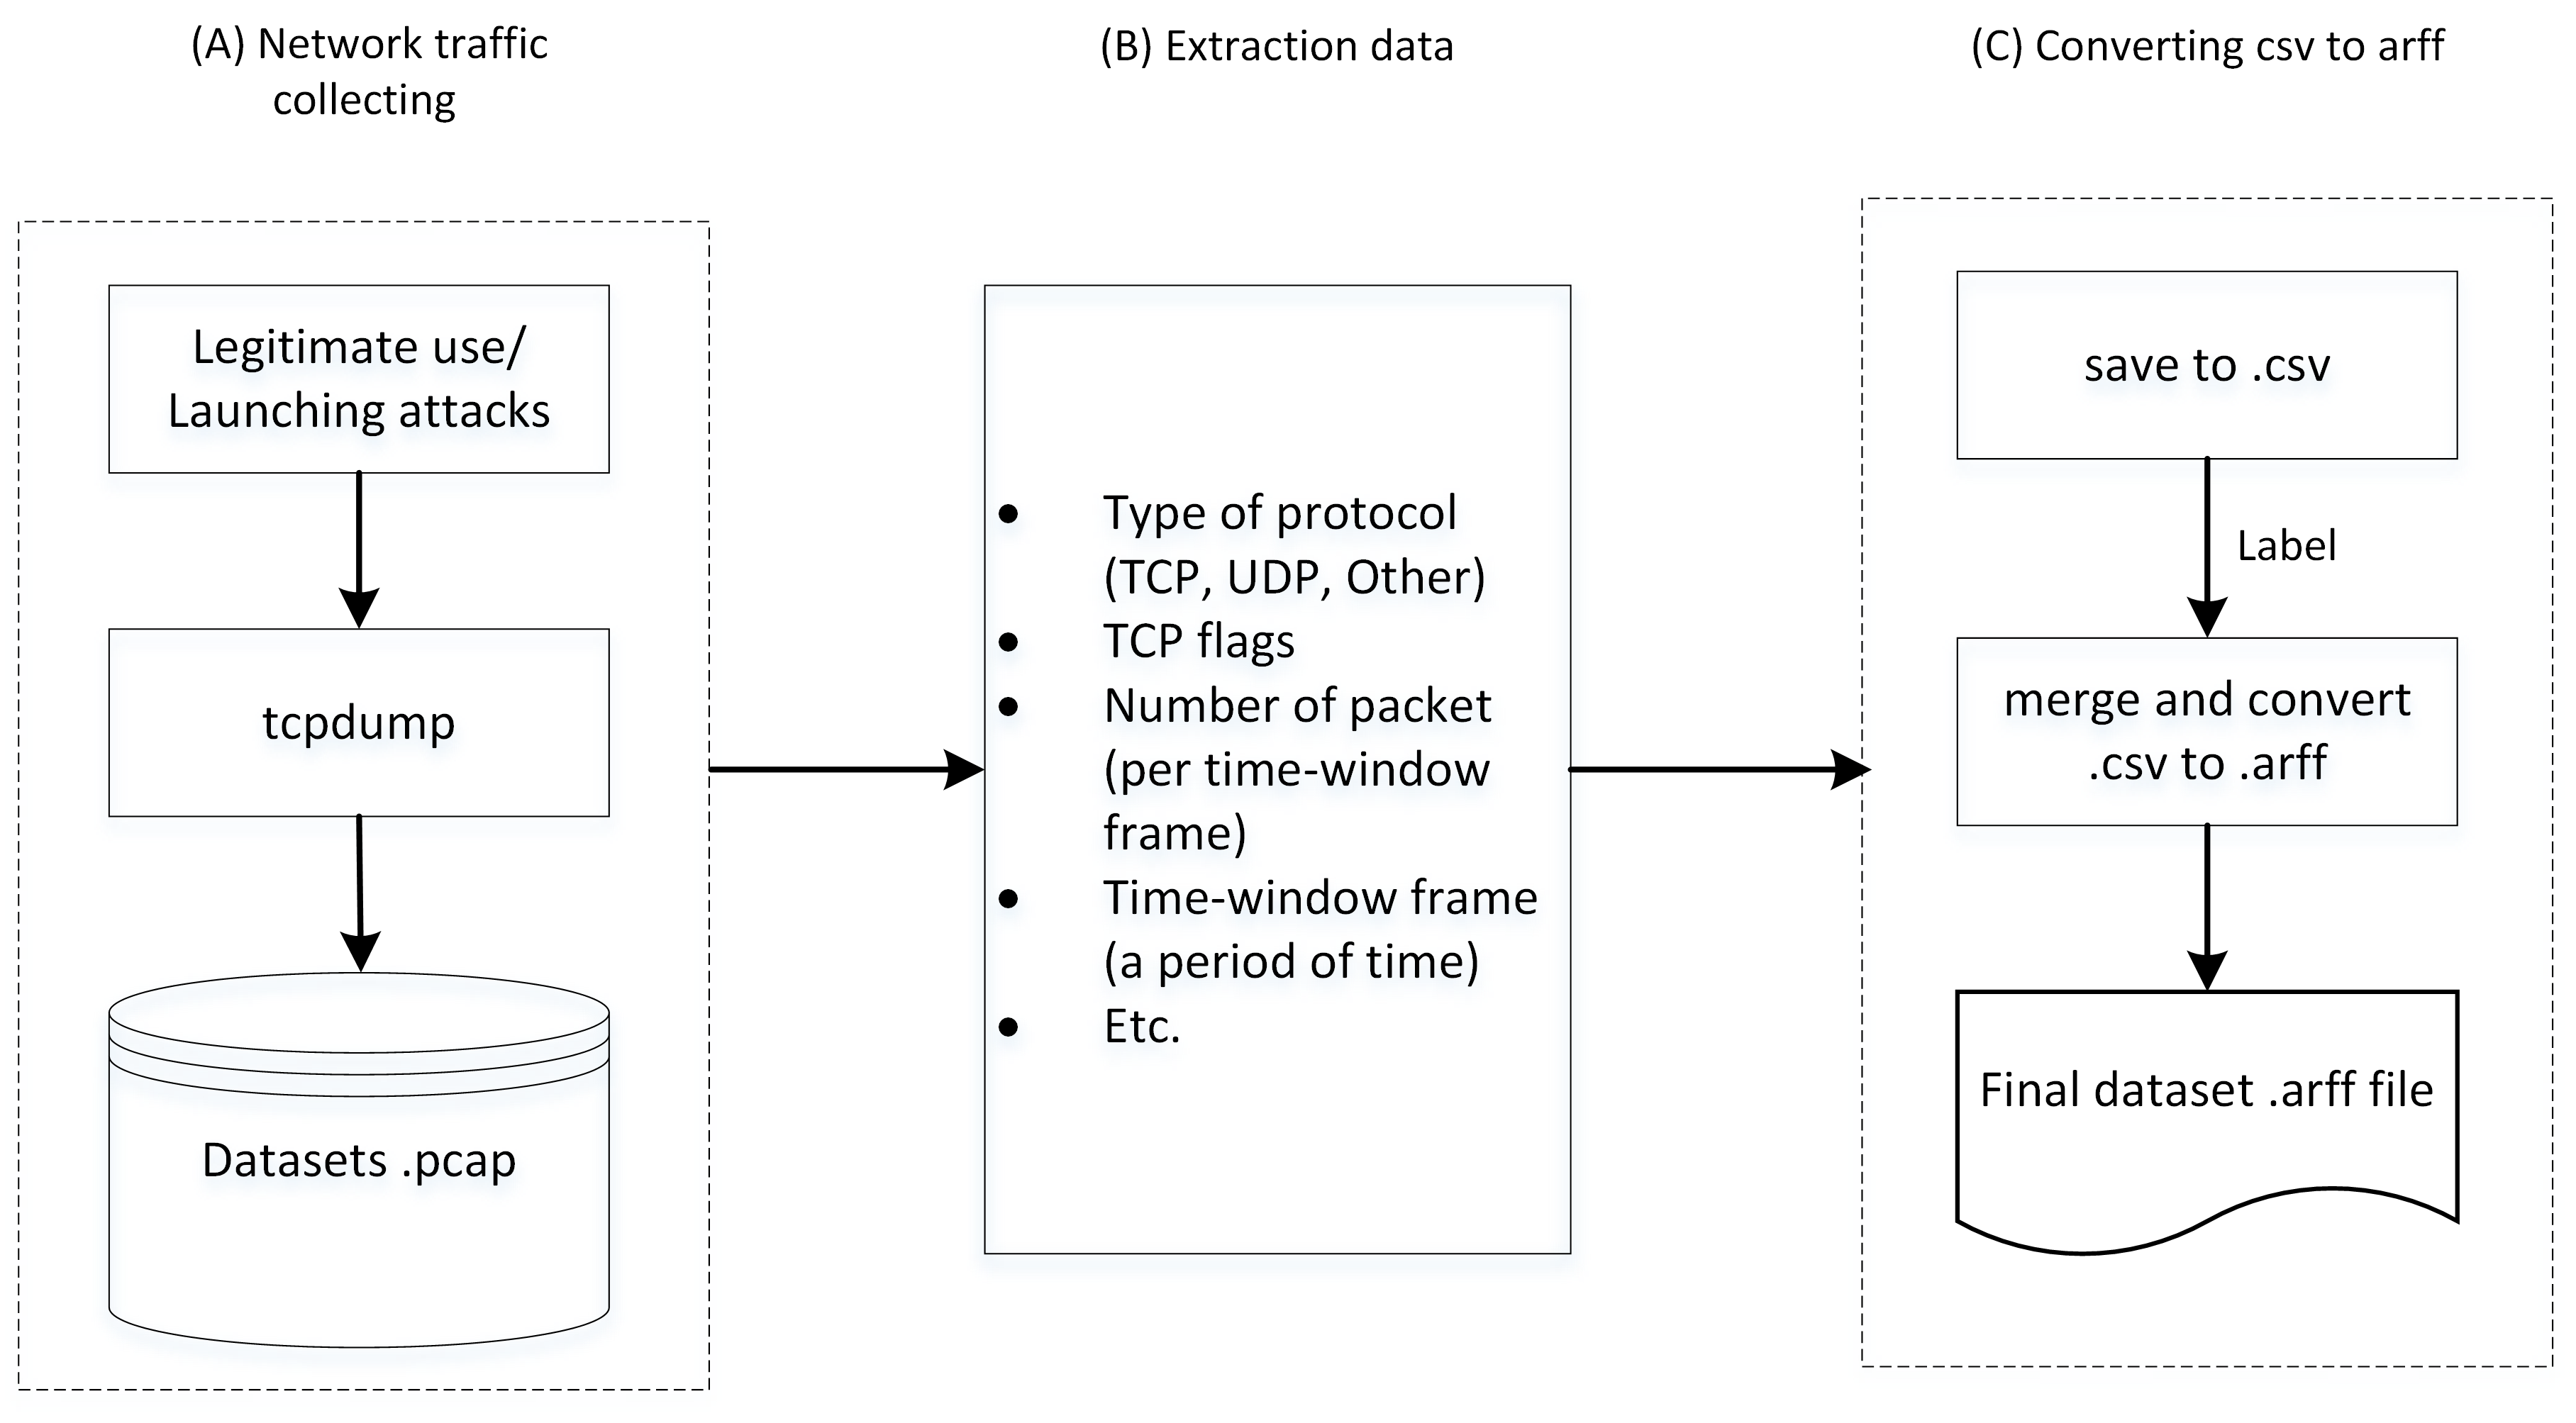
\includegraphics[width=\linewidth]{dataset_preparation_no_background.png}
\caption{Process of dataset preparation}
\label{fig:dataset_prepare}
\end{figure}

\noindent Each row into the final Csv represents a unique direction from source\_ip to destination\_ip for 4sec time window. List of features which we covered into dataset is shown in the Table \ref{table:features} and the dataset preparation process is shown as Figure \ref{fig:dataset_prepare}.

\begin{table}
\begin{center}
\begin{tabular}{|p{3.1cm}|p{4.9cm}|}
\hline
\multicolumn{1}{|c|}{\bfseries Name of Feature} & \multicolumn{1}{c|}{\bfseries Description}\\
\hline
TYPE\_PACKET & Which type of packet – tcp, udp and other into string\\
\hline
FIRST\_TIMESTAMP & Arriving timestamp when the first packet received into numeric\\
\hline
NO\_OF\_PACKETS & No of packets how much received into numeric\\
\hline
DEST\_IP & Destination IP into string\\
\hline
SOURCE\_IP & Source IP into string\\
\hline
TCP\_FIN & Sum of TCP FIN flags into numeric\\
\hline
TCP\_SYN & Sum of TCP SYN flags into numeric\\
\hline
TCP\_RST & Sum of TCP RST flags into numeric\\
\hline
TCP\_PSH & Sum of TCP PSH flags into numeric\\
\hline
TCP\_ACK & Sum of TCP ACK flags into numeric\\
\hline
TCP\_URG & Sum of TCP URG flags into numeric\\
\hline
TCP\_ECE & Sum of TCP ECE flags into numeric\\
\hline
TCP\_CWR & Sum of TCP CWR flags into numeric\\
\hline
ETHER\_TYPE\_AVG & Average of Ethernet type into numeric\\
\hline
WIRELEN\_AVG & Average of Ethernet Wirelen into numeric\\
\hline
IP\_OFFSET\_AVG & Average of IP Offset value into numeric\\
\hline
IP\_LENGTH\_AVG & Average of IP Length value into numeric\\
\hline
IP\_VER\_AVG & Average of IP Version value into numeric\\
\hline
IP\_HLEN\_AVG & Average of IP hlen value into numeric\\
\hline
IP\_TTL\_AVG & Average of IP ttl value into numeric\\
\hline
IP\_FLAG\_AVG & Average of IP flag value into numeric\\
\hline
IP\_TYPE\_AVG & Average of IP type value into numeric\\
\hline
TCP\_OFFSET\_AVG & Average of TCP Offset value into numeric\\
\hline
TCP\_LENGTH\_AVG & Average of TCP Length value into numeric\\
\hline
TCP\_HLEN\_AVG & Average of TCP hlen value into numeric\\
\hline
TCP\_RESERVE\_AVG & Average of TCP Reserve value into numeric\\
\hline
TCP\_WINDOW\_AVG & Average of TCP Window size value into numeric\\
\hline
TCP\_URGENT\_AVG & Average of TCP Urgent value into numeric\\
\hline
PAYLOAD\_OFFSET\_AVG & Average of Payload Offset value into numeric\\
\hline
PAYLOAD\_LENGTH\_AVG & Average of Payload Length value into numeric\\
\hline
ANOMALY\_SCORE & Class feature to label pattern (NORMAL/NMAP/DOS/R2L)\\
\hline
\end{tabular}
\end{center}
\caption{Table of feature extraction}
\label{table:features}
\end{table}

\noindent We added time window size parameter flexible that in future one can change this parameter for their use by observing network traffic. We launched each attacks from attacker's machine and we assume that all the packets which are coming from that attacker's machine as an attack and then we labeled our dataset manually attacks and normal and converted into arff file format for development. We ignore and remove SOURCE\_IP, DESTINATION\_IP, and FIRST\_TIMESTAMP because we observe it somehow classified pattern by taking those specific values. So after removed those features we are just looking at network behavioral features and extracting those to classify and generate snort rule dynamically for matched patterns.



\subsection{Data modeling and Machine learning}

Weka library is one of the famous open source library for data mining and machine learning \cite{misc:wekaTutorial}. It provides various algorithm and methods to work on any types of dataset to extract useful features which can applies to identify more accurately and our research Began with dataset preparation to build and train our model. We used ANOMALY\_SCORE class variable to predict a specific pattern for normal or attack into dataset. Decision tree is used where dataset has some predictor by which pattern can be classified into appropriate class. In our research we used J48 algorithm which is easy to convert into conditional algorithm for automatic snort rule generation \cite{misc:weka.jar}. We used weka.jar library to implement J48 decision tree java program. Conditional program generated through weka by taking labeled training dataset as an input. It uses program template in which we designed snort rule template with weka static method call which takes labeled/unlabeled testing dataset and generates snort rules by looking at matched attack patterns and its classified feature values..

We used J48 decision tree machine learning algorithm to train the model as well as snort rule generation by using that model \cite{NIDusingDT}. J48 decision tree classifier classify pattern by number of feature from our dataset which we than converted into snort rule using snort rule template. For example if model classified a specific attack pattern by tcp\_syn, no\_packets and type\_packet features than it will put those values of that specific features into snort rule template which we used into our Java application and as an output of that program we get snort rules.

%alert tcp \$EXTERNAL\_NET any -$>$ \$HOME\_NET any (msg: "[*] Attack-detected on S"; flags: S; flow: from\_client; threshold: type both, track by\_dst, count 182765, %seconds 4; sid: 3000001 ;)


\subsection{Snort configuration}

Intrusion Detection System (IDS) is a device which monitors packets on your network. IDS reports attack behaviors based on rules and signatures applied to the machine. IPS could achieve Real-time intercepting by leveraging in-line deployment in the network. It analyzes all network traffic passing through interface and takes actions to suspicious packets immediately\cite{misc:netfilter}.

We converted Snort IDS into INLINE QUEUE mode by using Iptables rule and Snort configurations. Now, it receives packets sent from the Net filter Queue with the help of the nfnetlink\_queue library, compares them with Snort signature rules and alert or drop if they match a rule, then finally sends them back to Net filter Queue where the Snort Inline tagged packets are dropped \cite{misc:netfilter}. An IPS (Intrusion Prevention System) where a packet matching a signature rule is blocked or modified.

In this case, the attacker will get the same information or fingerprints as the responses from the Vulnerable when the Attacker scans vulnerability services on the victim which are fake responses (replaced payload packets). For example, the attacker gets a fingerprint of version of SSH service from the Vulnerable as SSH-2.0-OpenSSH-4.7p1 and gets the same information, SSH-2.0-OpenSSH-4.7p1, from Victim as well even though the corrected information is SSH-2.0-OpenSSH-6.6.1p1.

%\begin{figure}[h!]
%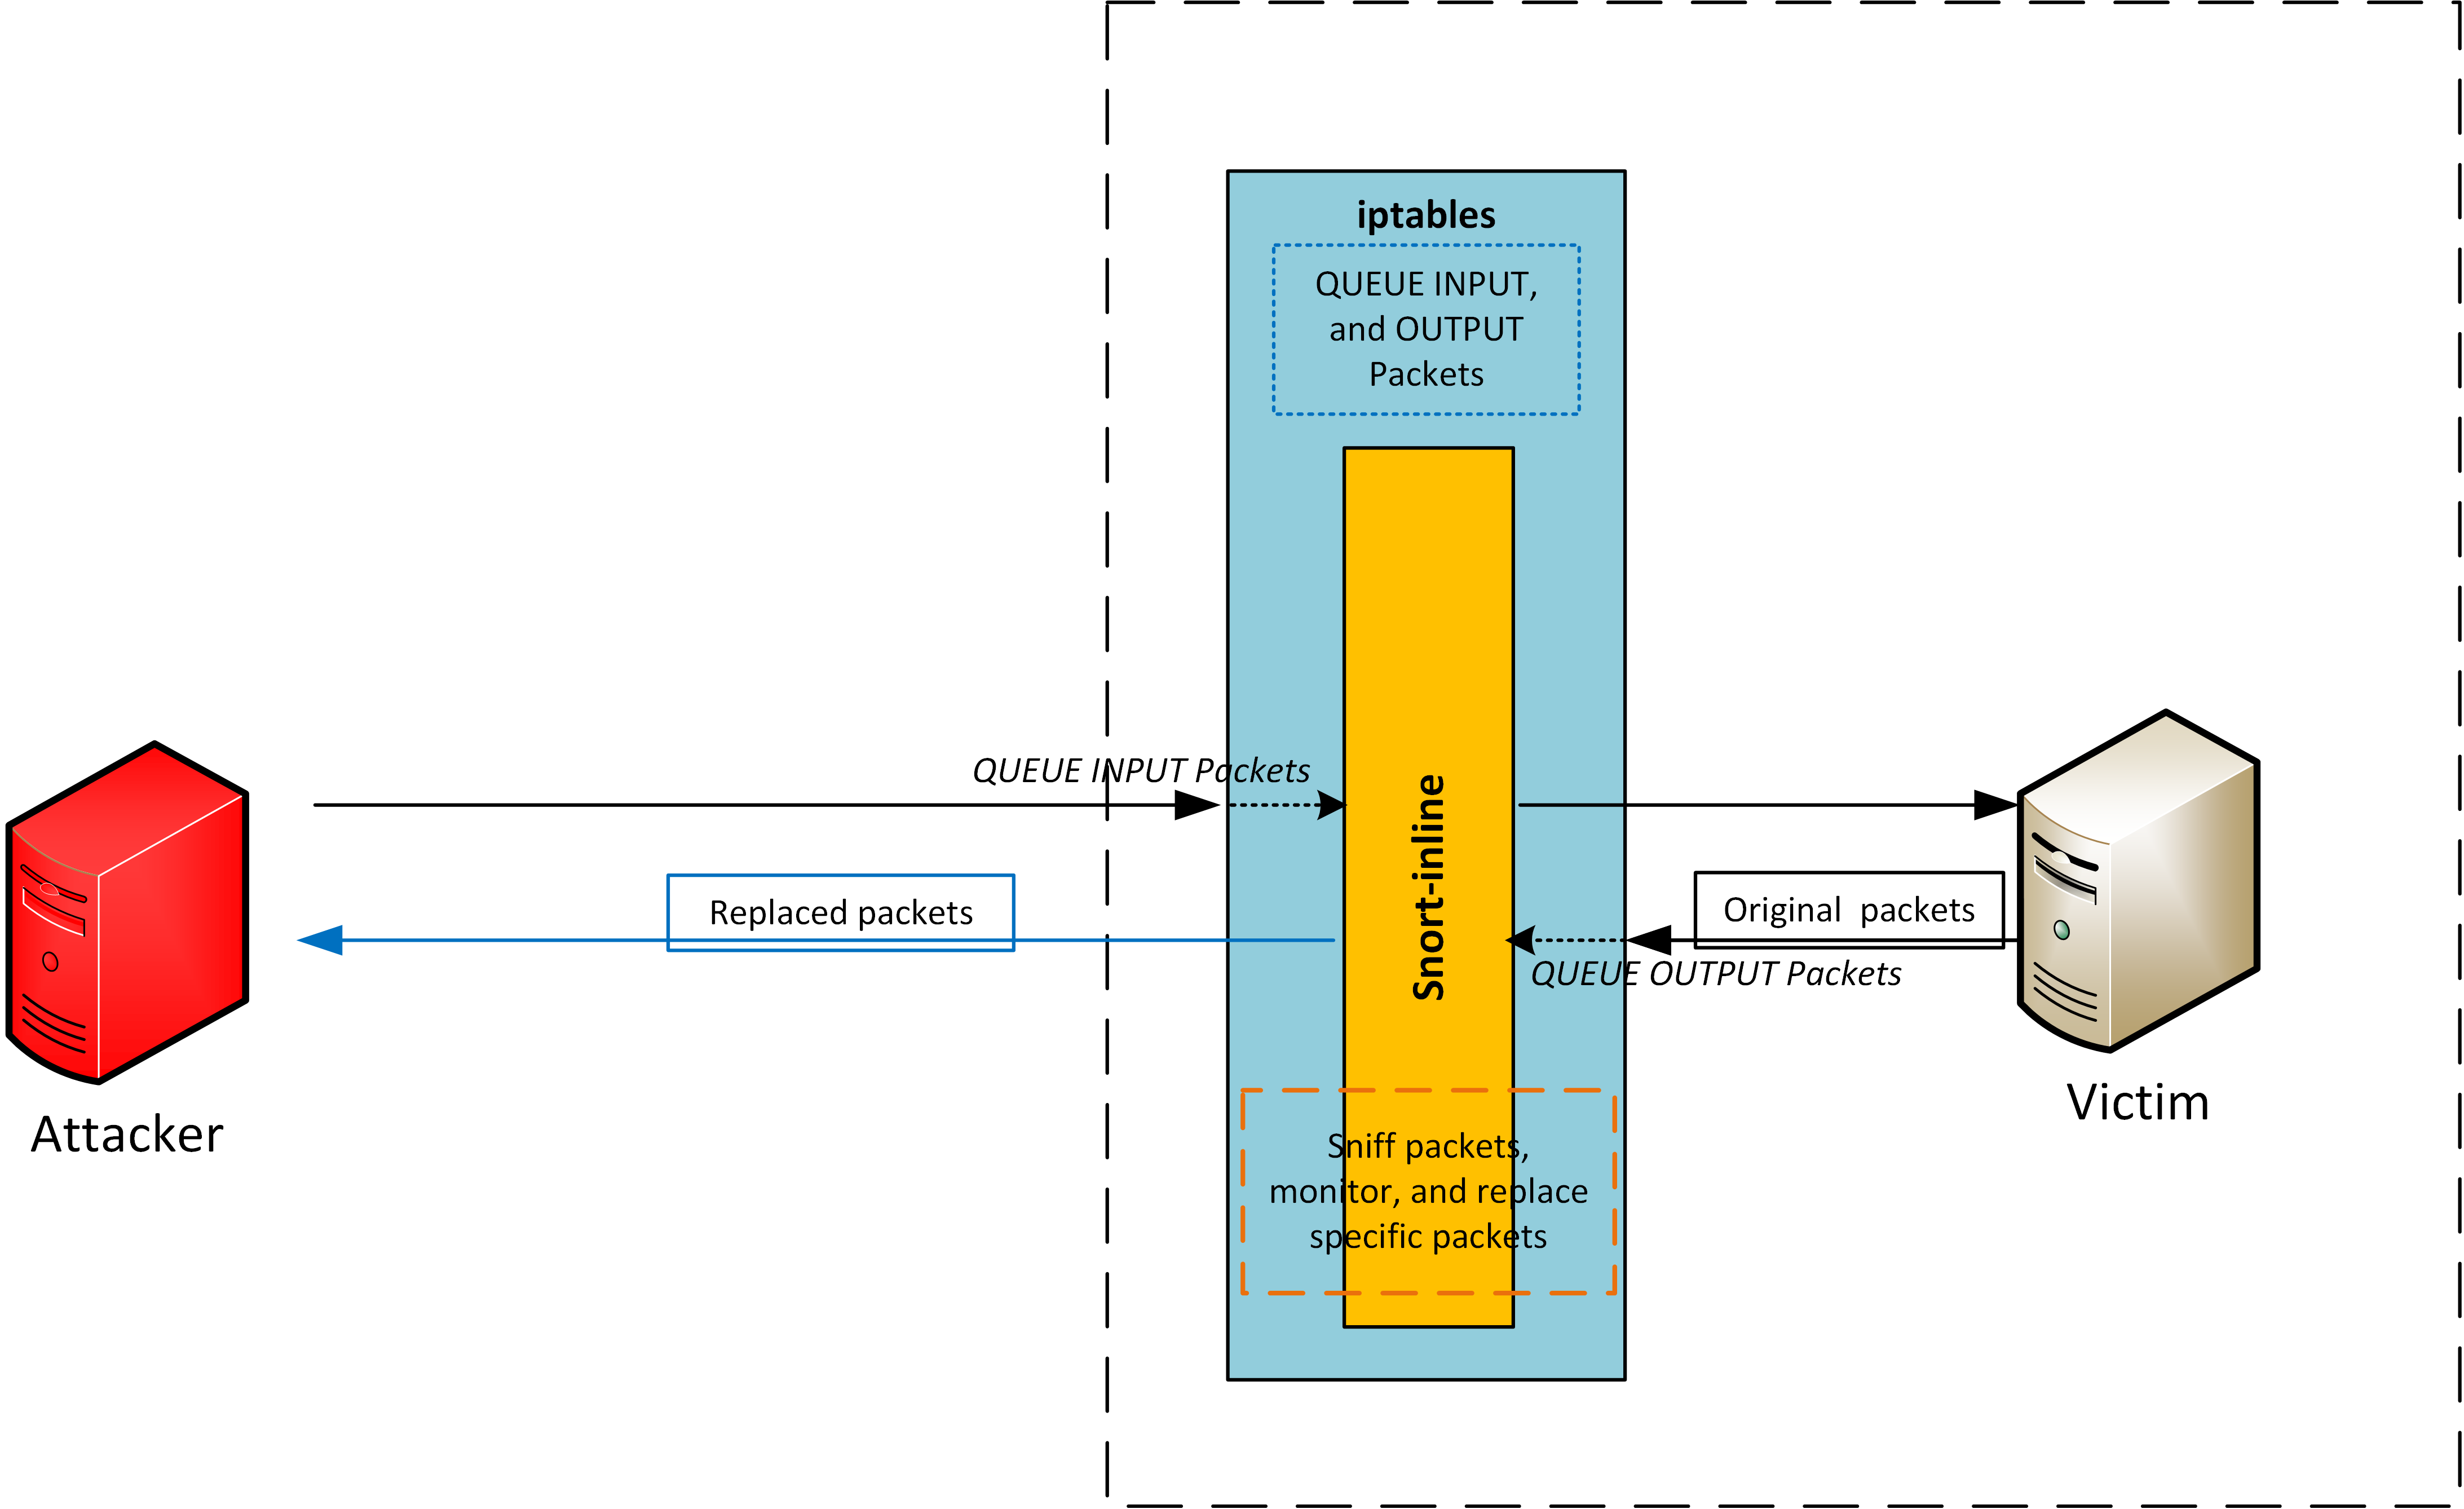
\includegraphics[width=\linewidth]{SnortProcessDiagram_no_back.png}
%\caption{Replacing payload model}
%\label{fig:replacementPayload}
%\end{figure}

%\noindent Figure \ref{fig:replacementPayload} shows how replacing process work on our model. 

In order to forge responses to service fingerprinting attempts, the first step is to queue all the packet not only from the attacker but also all the ingress/egress traffic by iptables. Then, all the traffic will pass through the snort which run as inline mode. The input traffic packets will not be replaced the payload, Snort just only monitor the traffic and try to match with the snort rule. Once the input packets are match with the rule, snort will replace the payload of the original output packet to be pre-payload which is same as vulnerable response. Lastly, the replaced packets that contain a fake response will be sent back to the attacker. Thus, the attacker will learn and get an incorrect information.

\subsection{Overall system setup}

The over-all process of N.A.D.I.R. system is show as Figure \ref{fig:overall}. As development phase of this research, we rebuild whole system by reconfiguring snort and adding snort rules to replace payloads by checking TCP flags of incoming requests \cite{misc:snortflowbit}. We divide snort rules into four different rule files: (1) my-flowbits.rules, (2) my-print.rules, (3) my-snort.rules, and (4) my-drop.rules

The (1) my-flowbits.rules and (2) my-print.rules which we developed at beginning are used to control the process of replacement of any string or payload. The other rule files will maintain by our Java application. At the end we come up with the overall system setup with our java application which takes training label set and once it will regenerate J48 decision tree algorithm by taking unlabeled testing sets or label instead  and it can generate snort rules dynamically. Java application generates snort rules and updates my-snort.rules file as per the training/testing dataset. Java application keep tracking on snort logs and it generates drop rule and update my-drop.rules file if an attack happened and detected. After successfully update snort rules, we managed deamon to restart snort service without missing any packet. We used two different deamon services and created two snort instances and handled two snort instances with two bridge interfaces. Here, if first snort instance is running and once snort rule updated, Java application runs another snort instance with updated rule sets and kill the first snort instance. The system flush entire drop rule file every night and keep the all blacklist IPs into backup file automatically. We tested our model step by step as well in real-time network traffic.
